\documentclass{article}
\usepackage[hmargin=0.65in, vmargin=0.65in]{geometry}
\usepackage[utf8]{inputenc}
%% \usepackage{indentfirst}
\usepackage{listings}
\usepackage{xcolor}
\usepackage{hyperref}
\hypersetup{
    colorlinks=true,
    linkcolor=blue,
    filecolor=magenta,      
    urlcolor=cyan
    }
\usepackage{graphicx}
\graphicspath{ {./images/} }


\title{CS 470 Homework 4}
\author{Niki Vasan}
\date{March 30th, 2023}

\begin{document}

\maketitle

\textbf{Collaboration Statement:} I pledge to abide by the Emory honor code. The only source I used in the completion of this assignment is the textbook, specifically Ch 5.1. I did not collaborate with any peers.


\section{Graph Test Cases} 
For this assignment, I created 5 graph test cases. 
\subsection{Graph 1}
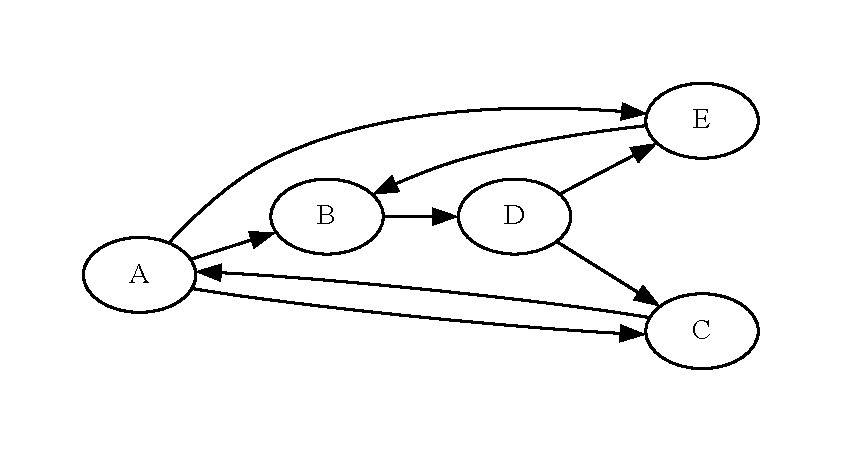
\includegraphics[scale=0.6]{graph1.jpg}
\newline
Graph 1 has 5 vertices with no spider traps or dead ends. All nodes have both an incoming edge and outgoing edge. Each potential loop has a node that has at least two outgoing edges to prevent a spider trap.
\subsection{Graph 2}
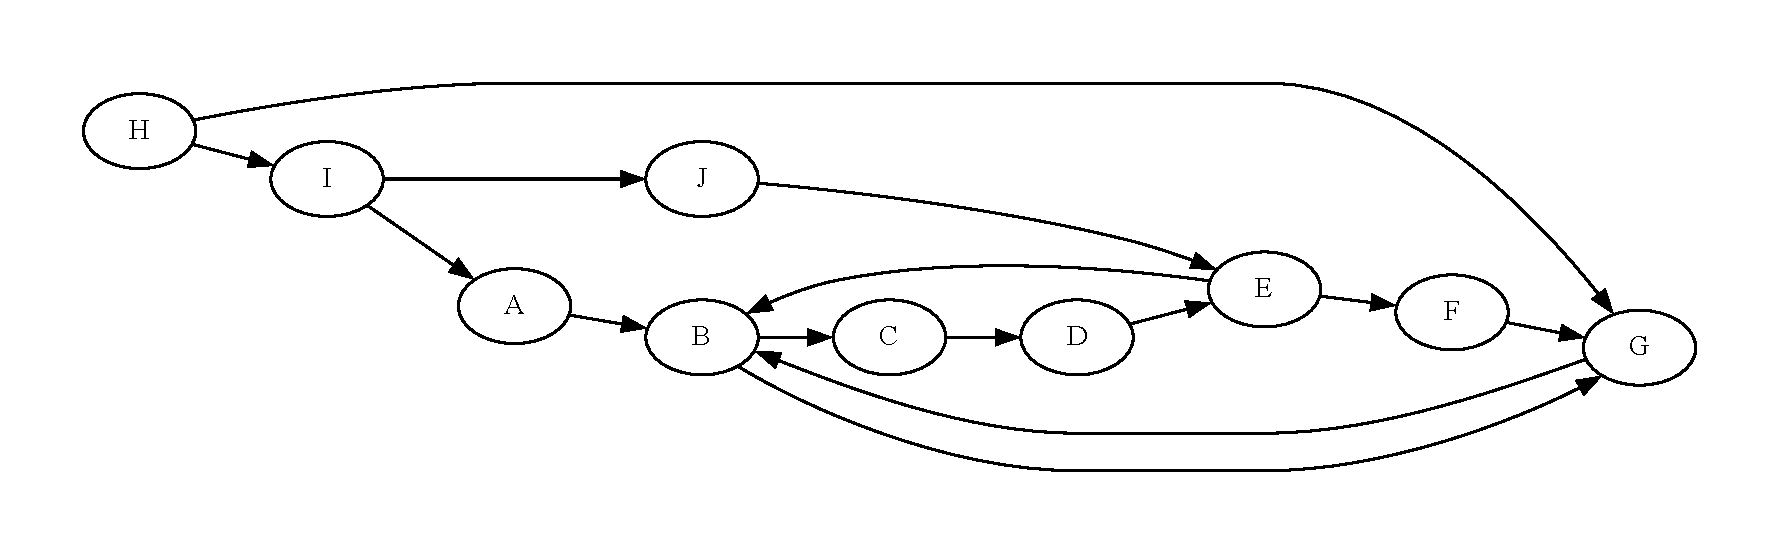
\includegraphics[scale=0.6]{HW4/graph2.png}
\newline
Graph 2 has 10 vertices with no spider traps or dead ends. The same explanation as Graph 1 applies. 
\subsection{Graph 3}
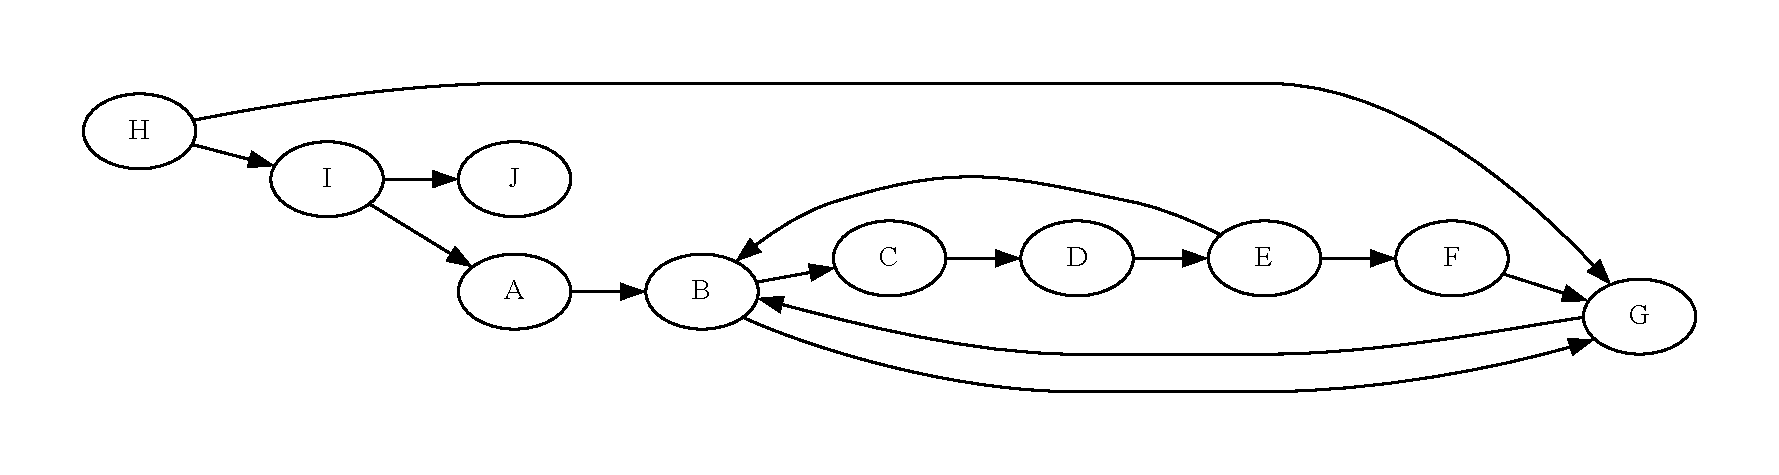
\includegraphics[scale=0.6]{HW4/graph3.png}
\newline
Graph 3 has 10 vertices with one dead end and no spider traps. Vertex J is a dead en in this graph, because it has no outgoing edges. 

\subsection{Graph 4}
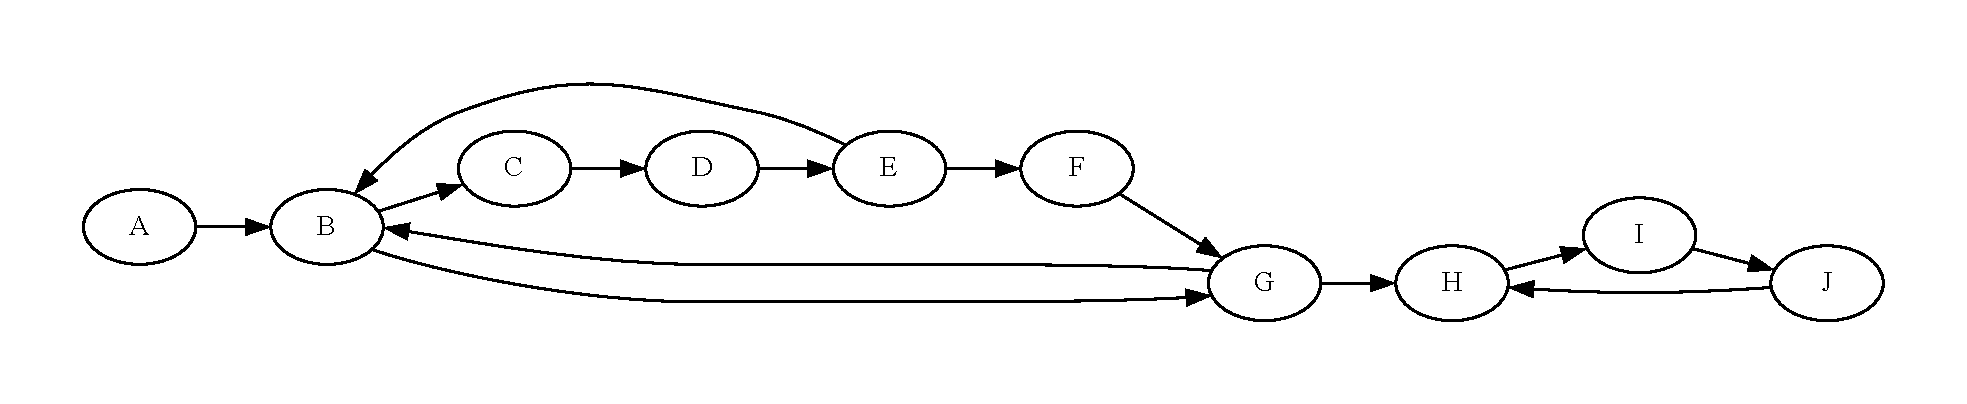
\includegraphics[scale=0.6]{HW4/graph4.png}
\newline
Graph 4 has 10 vertices with no dead ends and one spider trap. Vertices H, I, J form a 3 node spider trap, because all outlinks of the nodes are within the group. 

\subsection{Graph 5}
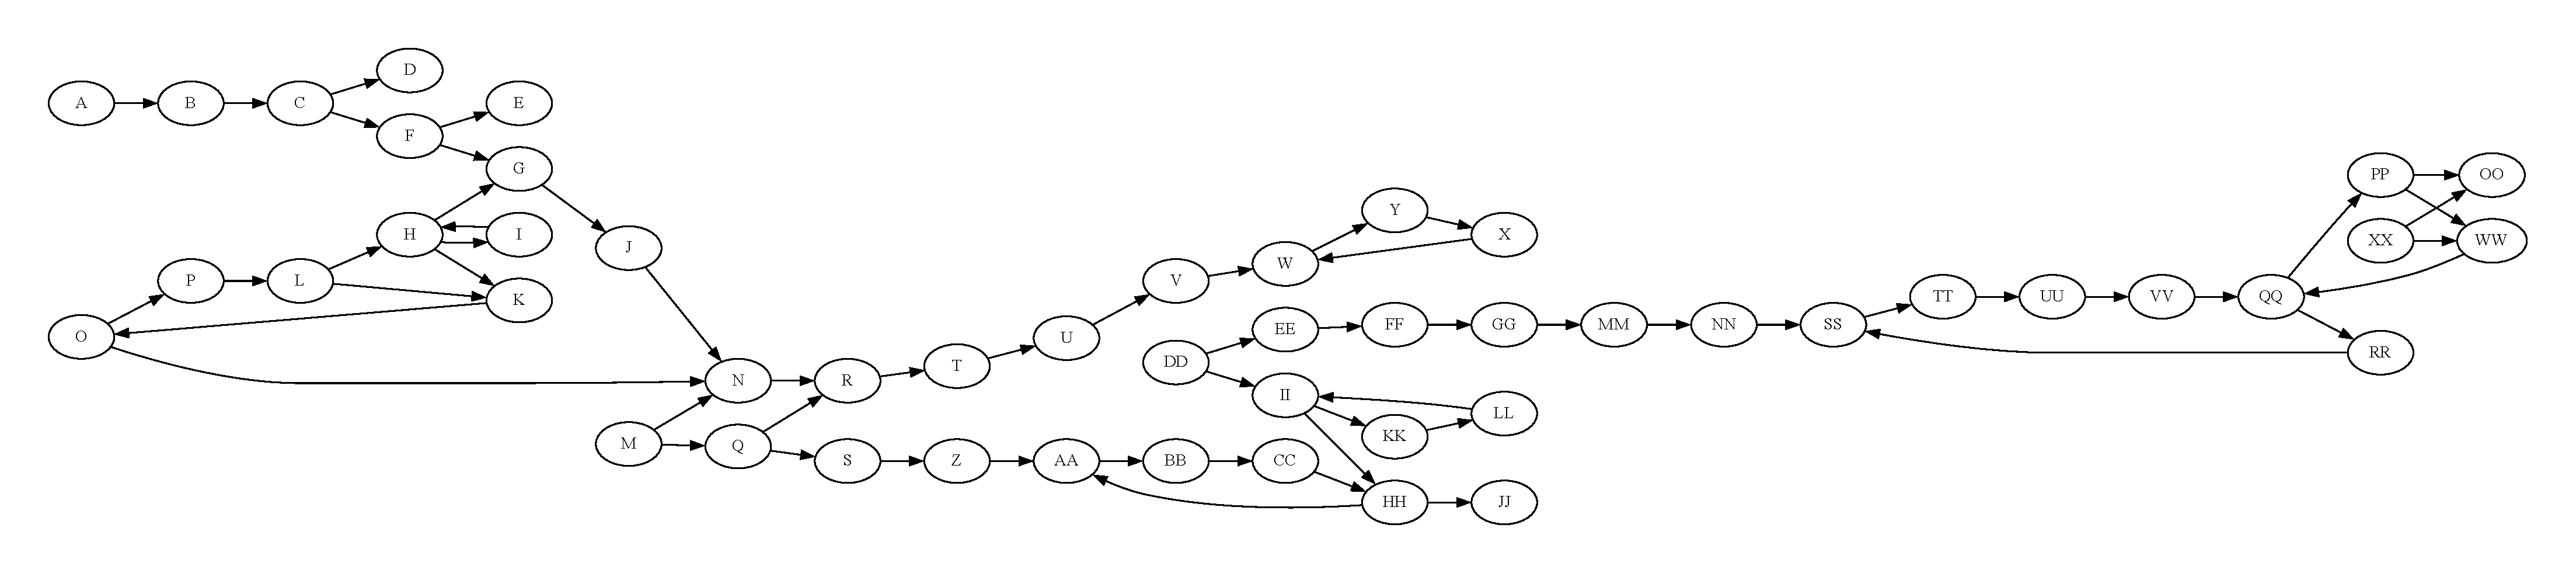
\includegraphics[scale=0.2]{HW4/graph5.png}
\newline
Graph 5 has 50 vertices with 4 dead ends and one spider traps. Nodes D, E, JJ and OO are dead ends because they contain no outgoing edges. Nodes W,X,Y form a spider trap.

\section{Page Rank Algorithm}
\subsection{Implementation}
\subsubsection{Data Structures}
I based my implementation of the algorithm off of the page rank formula provided in Ch 5.1 of the textbook. I first read in the input graph DOT file as a string and add each node-edge pairing to a list of tuples. To store the graph itself, I use a `defaultdictionary` where the keys represent parent nodes and their "children" (outgoing edges) are stored as values. Because the input node values are letters of the alphabet, I create a node mapping dictionary that stores each node with a unique index. Using this mapping, I transform the graph to be represented using integer indices, which is easier to work with for my implementation. 
\subsubsection{Transition Probability Matrix}
After the data is stored in an integer-represented graph, I create the transition probability matrix M. I initialize an nxn 2D array, where n = number of nodes in the graph. For each row in the matrix, if the node is not a dead end, I retrieve the indices of its outgoing edges and populate the respective column indices with probability 1/o (where o=number of outgoing edges). If the node is a dead end, that means it is not represented as a key in the graph and has no outgoing edges. This means all probabilities will be 0. Finally, I transpose this matrix to create M. 
\subsubsection{Updating Page Rank}
The textbook formula for page rank with a teleportation factor is: $\beta M \vec{v} + (1-\beta)\vec{e}/n$, where M is the transition probability matrix created earlier, v is the pagerank vector, beta is the teleportation factor (default = 0.8) and e is a vector of ones with length n. I used numpy arrays and matrices to achieve this multiplication. To update the page rank, I kept track of the current rank vector and the previous rank vector. 
The terminal condition of the algorithm is if the current and previous vector are equal, or if the absolute value of the element wise difference between the two is less than a specified convergence threshold, which I set to 0.0001. I made this condition because numpy vector equality checks if each digit in each element is the same, including digits that are not visible. My options were to truncate the numbers in each iteration or to set a threshold for equality. 
\subsubsection{Dead Ends and Spider Traps}
The dead ends and spider traps were handled with the teleportation factor. This is the probability that a surfer will randomly jump to a new node. This is not a completely foolproof solution, as nodes in spider traps still tend to have higher page rank scores, but the algorithm does converge. 

\section{Results}
Here are the output CSVs for each of the graphs listed above. The results for graph 5 are not listed for the sake of space (it has 50 nodes), but the csv can be found in the directory.  The rest of the CSVs, input DOT files and pdfs of graphs can be found in the directory as well.
% Graph 1
\begin{table}[ht!]
    \centering
        \begin{tabular}{| c | c |}
        \hline
        Vertex & Pagerank \\
        \hline
        B & 0.23 \\ 
        \hline
        D & 0.224 \\ 
        \hline
        A & 0.182 \\
        \hline
        C & 0.178 \\
        \hline
        E & 0.178 \\
        \hline
        \end{tabular} \\
        \caption{Graph 1 Output}
\end{table}
% Graph 2
\begin{table}[ht!]
    \centering
        \begin{tabular}{| c | c |}
        \hline
        Vertex & Pagerank \\
        \hline
        B & 0.251 \\ 
        \hline
        G & 0.189 \\ 
        \hline
        E & 0.138 \\
        \hline
        C & 0.12 \\
        \hline
        D & 0.116 \\
        \hline
        F & 0.075 \\ 
        \hline
        A & 0.031 \\ 
        \hline
        J & 0.031 \\
        \hline
        I & 0.028 \\
        \hline
        H & 0.02 \\
        \hline
        \end{tabular} \\
        \caption{Graph 2 Output}
\end{table}
% Graph 3
\begin{table}[ht!]
    \centering
        \begin{tabular}{| c | c |}
        \hline
        Vertex & Pagerank \\
        \hline
        B & 0.219 \\ 
        \hline
        G & 0.165 \\ 
        \hline
        C & 0.108 \\
        \hline
        D & 0.106 \\
        \hline
        E & 0.105 \\
        \hline
        F & 0.062 \\ 
        \hline
        A & 0.031 \\ 
        \hline
        J & 0.031 \\
        \hline
        I & 0.028 \\
        \hline
        H & 0.02 \\
        \hline
        \end{tabular} \\
        \caption{Graph 3 Output}
\end{table}

% Graph 4
\begin{table}[ht!]
    \centering
        \begin{tabular}{| c | c |}
        \hline
        Vertex & Pagerank \\
        \hline
        H & 0.185 \\ 
        \hline
        I & 0.168 \\ 
        \hline
        J & 0.154 \\
        \hline
        B & 0.108 \\
        \hline
        G & 0.104 \\
        \hline
        E & 0.076 \\ 
        \hline
        D & 0.071 \\ 
        \hline
        C & 0.063 \\
        \hline
        F & 0.051 \\
        \hline
        A & 0.02 \\
        \hline
        \end{tabular} \\
        \caption{Graph 4 Output}
\end{table}


\section{Insights + Lessons Learned}
In this assignment, I learned how to handle edge cases efficiently and effectively. Translating the formula from the textbook into code was relatively straightforward, but it required some thinking to account for dead ends while using a dictionary to store the graph, for example, or figuring out that array equality checks impact convergence. 

\end{document}
